\chapter{鲁棒性}
\label{chap:trust-robustness}

一个邮件分类器通过了旧月份的测试，到了新月份却频繁误拦正常邮件。要定位问题，先得看这一个月里究竟是什么变了。一种变化发生在测量环节：同一封邮件换了压缩方式，或网关的 OCR 版本升级，模型读到的像素、字符与旧版本不同，但邮件是不是垃圾邮件并没有改变。另一种变化发生在规律本身：正常业务也开始采用过去只在垃圾邮件里出现的模板，于是“带某个页脚就是垃圾邮件”这条旧规律不再成立。前者只要求模型对同一封信的不同呈现保持判断，后者则要求模型识别并学习已经改变的规律。两类问题需要的证据和补救完全不同，所以谈“模型稳不稳”之前，必须先回答：部署时究竟要求它承受哪些变化。

\term{鲁棒性}（robustness）刻画的正是这个问题：在事先规定的变化范围内，模型能否继续完成任务。注意它不是一句笼统的“抗干扰能力强”，任何一条鲁棒性主张都必须写清三件事——变化的对象（输入测量、群体比例，还是特征与标签的关系）、变化的范围（允许多大噪声、哪些环境），以及衡量表现的指标和最低标准。若模型已经失效、或现有数据不足以给出判断，部署系统还应能识别异常输入、拒绝自动处理或回退到人工，把损害控制住；这一层能力称为\term{变化应对能力}（resilience to change）。两者评价的对象不同：鲁棒性回答“模型在变化中还准不准”，变化应对回答“模型不可靠时系统会不会闯祸”。围绕这两个问题，本章给出四类工具。变化风险用测试集估计总体性能，局部认证则对每一个具体输入证明其附近不会翻转；识别、拒绝和回退评价系统怎样在范围外止损；训练约束改变模型在已知变化下的行为，利用新环境信息更新模型，限制自动处理范围则缩小一旦出错可能造成的损害。第~\ref{chap:transfer-learning-theory}章给出变化下“哪些规律可学”的条件，本章把这些条件接到具体的检验与改进方法上。

这一安排与第~\ref{chap:trust-foundations}章的三层框架对应：要求层在这里规定允许改变哪些条件，以及变化后任务风险或表现至少要满足什么标准。没有这项声明，“稳健”就没有确定的评价对象——对压缩鲁棒、对模板更换鲁棒和对全新诈骗类型鲁棒，是三个完全不同的承诺。

它也与上一章紧密衔接。上一章的校准、覆盖和风险保证都建立在“数据与未来输入满足某种关系”（如可交换、独立同分布）之上；关系一旦改变，这些主张就可能失效。本章先检查关系改变后哪些证据仍然有效，再讨论模型或数据来源持续变化时，如何监测、触发、回退和复验。要求、证据和生命周期条件由此共同限定鲁棒性。

最后说明一点：允许的变化既可能来自测量误差和自然环境，也可能由对手主动寻找。本章只按“允许集合加损失”的抽象形式讨论局部方法；到第~\ref{chap:trust-security}章，还会加入攻击者的权限、资源和损害路径。测量误差与对抗扰动可以共用同一套局部稳定性工具，但完整的安全问题还涉及数据、模型、系统等更多环节。

\section{模型的鲁棒性}
\label{sec:robustness-fragility}

要系统地回答“模型在变化中表现如何”，先把两件事分开。第一是变化范围：部署时允许哪些输入或环境发生变化，这决定了应该测试什么。第二是失效机制：模型为什么会在这些变化中出错，这决定了应该怎样补救。二者不是一一对应的：同一种变化（如附件压缩）可能因不同机制导致失败，同一条脆弱规律（如依赖页脚）也可能被多种不同变化暴露。本节先界定范围，再分析机制。

\subsection{变化范围与性能要求}
\label{sec:robustness-change-scope}

先考虑最简单的一类变化：邮件的正确标签不变，只是它在模型眼里的呈现可以改变。固定参考邮件总体$\mathcal P$与预测器$f$。对每封邮件，任务规定一个非空的允许集合$U(\bm{x})$，它包含原输入$\bm{x}$本身，集合中的每个变体$\bm{x}'$都代表同一封邮件、正确标签仍是$y$。它可以由任务直接给出：对图像是“像素改动不超过某个半径”，对文本是“同义改写或 OCR 误识的可能形式”，对邮件是“允许的压缩和编码差异”。设损失$\ell$越大表示预测越差。如果要求模型在允许集合内的每一个变体上都不能出错，评价时就要先对集合内的损失取上确界（最坏的那个变体），再对参考总体平均：
\begin{equation}
 R_{\mathrm{pert}}(f)
 =\mathbb E_{(\bm{x},y)\sim\mathcal P}
   \left[\sup_{\bm{x}'\in U(\bm{x})}
   \ell(f(\bm{x}'),y)\right].
 \label{eq:robustness-perturbation-risk}
\end{equation}
这里为什么用“上确界”而不是对扰动再取一次平均？因为对扰动随机抽样只能描述“平均加噪后错多少”，有可能漏掉少数改动很小却让模型彻底翻转的点；而上确界对应一个全称要求——只要允许集合里存在一个错误变体，这封邮件就不算通过。预设一个容限$\rho_{\mathrm{pert}}$后，可以要求$R_{\mathrm{pert}}(f)\leq\rho_{\mathrm{pert}}$。需要强调，哪些变化可以进入$U$完全由任务决定：像素噪声、等义改写、测量误差都可以，但删除否定词这类改动虽然只动几个字符，却真的改变了邮件含义和标签，就不能要求模型对它保持原输出。

式~\eqref{eq:robustness-perturbation-risk}有一个局限：外层总体$\mathcal P$始终没变，变化只发生在单封邮件的邻域内。新月份带来的往往不是这种局部改动，而是整个人群的构成、乃至特征与标签的关系都变了。为描述这种变化，需要引入环境集合$\mathcal E$：每个环境$e\in\mathcal E$对应一个数据分布$\mathcal P_e$，参考环境记为$0\in\mathcal E$且$\mathcal P_0=\mathcal P$，模型在该环境中的风险为$R_e(f)=\mathbb E_{(\bm{x},y)\sim\mathcal P_e}\ell(f(\bm{x}),y)$。环境集合应声明允许改变什么：各类邮件的比例、标签比例、输入的边缘分布，还是给定输入后的标签规律，具体类型见第~\ref{sec:distribution-shift}节。在此基础上可以提出两种不同要求：约束最坏环境的风险水平$\sup_{e\in\mathcal E}R_e(f)\leq\rho$，或约束相对参考环境最多恶化多少$\sup_{e\in\mathcal E}[R_e(f)-R_0(f)]\leq\delta$。这两个数回答不同问题，必须一起报告：一个本来就很差的模型在新环境中可能恶化很小，风险水平却始终不可接受。还要注意，局部邻域证书通常推不出这两个环境层面的保证。

\begin{example}[总体表现掩盖群体脆弱性]
\label{ex:robustness-mixture}
构造一个旧环境：99\%的邮件使用常见模板，模型在这类邮件上的错误率只有1\%；另有1\%的邮件使用少见模板，模型对它们的错误率高达50\%。按各组所占比例加权，总体错误率只有
\[0.99\times0.01+0.01\times0.5=0.0149\text{，}\]
即1.49\%，看起来相当好。到了新环境，模型本身和它在每一类邮件上的表现都没有任何变化，只是少见模板的比例从1\%提高到30\%，总体错误率便变成
\[0.70\times0.01+0.30\times0.5=0.157\text{，}\]
即15.7\%。这个例子说明一个重要事实：即使模型的参数没有变、它在每个组内的标签规律也没有变，仅仅是各群体比例的改变，就足以让总体表现大幅退化。只看一个总体平均数字，会把这种脆弱性完全掩盖掉。
\end{example}

图~\ref{fig:trust-robust-neighborhood}把本章检验部分要用到的两种动作画在一起。允许集合中的一个错误变体，就足以反驳“这封邮件在整个邻域都正确”的全称主张；但要对总体容限下结论，还必须按参考样本的抽样方式把逐样本结果聚合起来。反过来，若想证明整个邻域都稳定，则需要一种能覆盖邻域中每一个点的认证依据，而不能只靠抽几个点试试。搜索反例、总体估计和邻域认证是三种不同对象，后面分别展开。

\begin{figure*}[!htb]
  \centering
  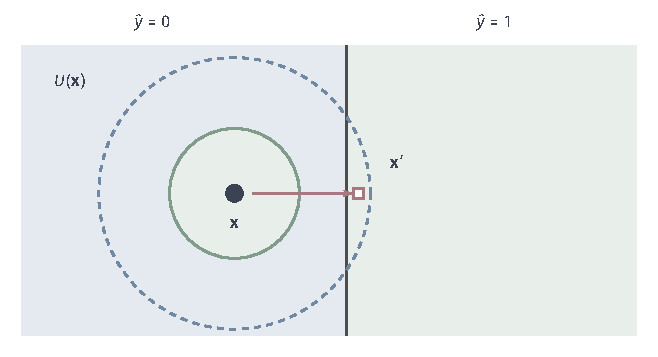
\includegraphics[width=111.404mm]{figures/03-foundations/03-trustworthiness/tikz/trust-robust-neighborhood/figure.pdf}
  \caption{虚线圈为允许集合$U(\bm x)$，内圈为已认证稳定范围，方点$\bm x^{\prime}$在允许集合中跨越决策边界。尺寸仅示意集合关系，未取自随机平滑实验。搜索无反例尚未认证全允许范围。}
  \label{fig:trust-robust-neighborhood}
\end{figure*}

\subsection{失效机制与信息缺口}
\label{sec:robustness-failure-mechanisms}

允许范围只告诉我们“测什么”，还没有解释“为什么会出错”。失效机制不同，补救需要的信息也不同。本章主要涉及三种机制：一是决策边界离输入太近，输入轻微改动就越过边界导致预测翻转；二是原本错误率就高的群体在新环境中占比变大，平均风险被抬高；三是特征与标签之间的联系本身改变，旧规则不再成立。示例~\ref{ex:robustness-mixture}属于第二种：它没有制造任何新的组内错误，只是给本来就困难的样本增加了权重。另外还要把这三种机制与标注错误、测量异常等数据质量问题区分开——这些情形应先核查记录的来源和含义，再决定修正数据、补充观测，还是采用适合该类污染的稳健损失或估计方法。不能只凭残差大就把合法困难样本当脏数据，也不能预先把修数据与改估计方法设成排他的选择。

第三种机制最隐蔽，需要从训练目标本身理解。如果训练时只最小化当前样本上的分类损失，那么目标函数奖励的只是“在训练条件下把这批样本分对”，它并不区分模型使用的关系能不能迁移到新条件。设想垃圾邮件长期带一个固定页脚，模型记住“有这个页脚就判垃圾邮件”，在旧月份可以稳定答对；一旦正常邮件也开始带这个页脚，旧依据立刻失效。\term{捷径学习}（shortcut learning）指的就是这种现象：模型学到一条在训练条件下有效、却不足以支撑预期迁移的规则。Geirhos 等用图像模型对背景和纹理的依赖系统说明了这类问题，并强调捷径的认定必须结合数据和评价条件，不能只凭特征“看起来不本质”下判断\scite{geirhos2020shortcut}。

页脚是不是捷径，最终取决于鲁棒性要求是否允许“页脚改变而类别保持”。在一个业务关系长期稳定的场景里，页脚完全可能是合法且高效的判别依据。判断捷径时要避免两种直觉错误：看起来直观易读的特征未必稳定（发件人显示名也可以被伪造），高维、抽象的特征也未必是捷径（它们可能确实承载因果信息），人工制定的规则同样会依赖过时的相关性。真正可靠的判定方式是实际改变这层关系、观察预测是否跟着错，只看特征外观无法替代检验。

可以用一个人为对照看清“随机留出为什么检验不出捷径”。设垃圾邮件中90\%使用模板甲，正常邮件中90\%使用模板乙，那么只读模板就能达到90\%的准确率；按原比例随机划分训练集和测试集，测试集保持同样的比例，模板规则在测试集上依然有90\%的准确率，问题完全暴露不出来。但如果在测试时把两种模板均衡地分配给两类（模板与标签脱钩），同一条规则的准确率立刻降到50\%，与抛硬币相当。这是为诊断构造的对照，并不说明所有模型都会去学模板；它说明的是：随机留出只检验了同一分布内的泛化，没有检验“模板改变后模型是否仍靠内容判断”这一不变性。

如果现有的有限环境里模板与标签始终同向出现，数据中就根本不存在排除捷径所需的信息，任何模型选择方法都无法凭空判断哪条关系更可靠。增加环境多样性才可能把它暴露出来，但多样性必须对准目标变化：同一模板的近重复邮件再多，也不增加对“模板脱钩”这一情形的覆盖。更极端地，如果现有资料完全无法区分目标域里的标签规律，那么无论模型多复杂、正则多精巧、无标签适应多积极，都不可能补出数据中不存在的信息；定理~\ref{thm:transfer-nonidentifiability}给出的正是这类不可识别边界。

还要避免把“输出不变”当成无条件的目标。鲁棒性要维持的是任务表现，而不是在任何情况下都给出相同答案。当真实标签关系确实改变时，坚持旧答案反而是错误：一个合法发件主体被接管后，发自同一地址的邮件性质可能已经不同，系统理应利用新证据改变判断。因此正确的表述是分层次的：只有在标签保持的变化上，才可以进一步要求预测不变；对标签关系本身的变化，需要的是及时发现并学习新规律，而不是顽固地保持稳定。

\section{鲁棒性的检验}
\label{sec:robustness-evaluation}

明确了变化范围和失效机制后，检验部分依次回答三个不同的问题：变化后任务风险究竟是多少；对指定的输入邻域，能否排除预测翻转；当输入落在检验范围之外时，系统能否识别出来并及时止损。前两个问题评价的是模型本身（用带标签测试或形式认证），第三个问题评价的是系统应对（监测、拒绝与回退）。需要特别强调，这三类证据之间没有互相蕴含关系：报警灵敏不代表邻域内稳定，邻域证书也不保证分布外能识别。因此它们必须一起提供，却要分别解释，不能用一个好结果代替其余承诺。

\subsection{变化条件下的风险检验}
\label{sec:robustness-risk-test}

变化条件下的风险检验，第一步不是选基准，而是回到要求层：这个系统部署后真正会遇到什么变化？测量扰动类测试应尽量保留任务语义，只改变噪声、分辨率、压缩或缺失程度；跨环境测试要用新的时间、来源或设备采集的数据；此外还要对预设关键群体做切片检查，防止总体平均掩盖局部问题。每一项测试都必须记录扰动强度、标签如何复核，以及它覆盖的变化范围，否则数字无法与鲁棒性主张对应。

测试数据的组织方式会影响结论能说明什么。对同一封邮件、同一张图生成多个配对变体，可以排除样本组成差异，把某个因素（如噪声强度）单独隔离出来；而直接采集真实新环境的数据，则保留了实际部署中多种因素的耦合。两者回答不同问题，不能互相替代：配对实验回答“这个因素单独有多大影响”，真实环境回答“所有因素一起作用时风险是多少”。此外，如果数据增强策略是看着测试结果挑选出来的，就必须另外预留一批环境或扰动组合做最终检验，否则测到的只是“对这套测试的适应”，而不是可迁移的改进。

损坏基准就是把“配对扰动”标准化，使不同模型的结果可以重复比较。ImageNet-C 预设了噪声、模糊、天气和数字处理等若干类损坏，并为每类规定从轻到重的强度等级；ImageNet-P 则考察连续小变化下预测是否稳定（例如视频帧轻微抖动时分类结果是否来回跳）\scite{hendrycks2019corruptions}。它们的价值在于让“在规定压力下表现如何”成为一个可比较的量，但证据范围严格限于这些已列明的损坏类型和强度，不能外推为“对所有自然变化甚至最坏变化都鲁棒”。

基准常给出归一化分数（如相对某个参考分类器的损坏错误率），读这类数字时要先弄清分母。归一化分数描述的是相对表现，不是部署时的真实错误率；而且按损坏类型等权平均，可以作为预先约定的平衡压力指标，不要求业务真的等概率遇到各类损坏；但若将它解释为部署平均风险，就须使用与实际发生比例匹配的权重。一个真实服务如果几乎只遇到压缩问题，那么把天气、噪声等类型等权平均得到的分数，未必对应实际收益。报告时应按损坏类型和强度分别分解，并连同干净输入上的结果一起给出，归一化数值才可解释。

WILDS 基准把另一类变化——数据来源的系统性差异——纳入标准任务：它的数据来自不同医院、不同相机位置、不同时间段和地理区域，并规定了按来源划分数据的方式与评价指标\scite{koh2021wilds}。它用同一批任务清楚地展示了两种留出的差别：在同一来源内随机留出，测的是相应来源分布上的泛化；按整个来源留出（如训练时完全没见过某家医院），测的才是迁移到新来源的能力。

% 为完整文献边注预留高度，避免它被前面的长作者列表挤出纸边。
\Needspace{45mm}
分布变化的影响有时先出现在概率上，然后才反映为分类错误：模型可能在一段时间内仍能分对大部分样本，却对正在出错的样本越来越自信。Ovadia 等在一系列受控分布变化中同时比较各种不确定性方法的准确率、概率评分和校准误差，把“错误变多”与“对错误过于自信”这两种退化分开评价\scite{ovadia2019uncertainty}。引用这类结论时仍要连同具体的变化类型和强度，不能据此断言某方法在任意变化下都更可靠。

邮件这类业务数据做时间划分时，要特别防止信息泄漏：同一封邮件的近重复版本、同一会话中的多封往来邮件，不能一部分进训练、一部分进测试，否则模型可以靠记忆而非泛化答对。划分单位应对准“未知因素”：目标是迁移到新机构，就按整个机构留出；目标是未来月份，就严格保留时间顺序，用旧月份训练、新月份测试。还要交代调参时能看到哪些环境：用目标域标签做模型选择，与目标域完全不可见，是两个根本不同的设定，后者难得多。

除了平均风险，还要对在部署前根据人群、来源或成本预先指定的关键组，分别报告风险、样本数和置信区间。小样本组上一个好看的低点估计，可能只是抽样波动，不足以确认可靠。示例~\ref{ex:robustness-mixture}还提示：要判断平均退化从何而来，必须同时报告各组组内错误率和各组所占比例，二者缺一不可。

把上面的要求写成可计算的估计量。在环境$e$中，从$\mathcal P_e$独立抽取$n_e$个既没有参与训练、也没有参与模型选择的带标签样本，分别估计该环境的风险和相对参考环境的变化：
\begin{equation}
 \begin{aligned}
 \widehat R_e(f)&=\frac{1}{n_e}\sum_{i=1}^{n_e}
       \ell(f(\bm{x}_{e,i}),y_{e,i}),\\
 \widehat\Delta_e&=\widehat R_e(f)-\widehat R_0(f),
 \end{aligned}
 \label{eq:robustness-environment-test}
\end{equation}
两个量分工不同：$\widehat R_e$回答“在这个环境中风险有多高”，$\widehat\Delta_e$回答“变化使风险增加了多少”。一个模型可能$\widehat R_e$很高但$\widehat\Delta_e$很小（本来就差），也可能$\widehat R_e$尚可但$\widehat\Delta_e$很大（对变化敏感）。报告时还要按变化强度和预设组进一步展开。统计上有几点必须处理：容限$\rho$应对照风险的置信上界判断，点估计碰巧达标并不够；会话、机构、时间上成簇的数据要采用与聚类结构匹配的抽样假设和区间，各组被抽中概率不同时要加权；同一原样本的多个变体或前后测量彼此相关，必须保留这种配对依赖，不能当成独立观测重复计数。最后，如果同时对多个环境、强度或组作出“都达标”的承诺，还要做多重比较的联合控制；只给逐项区间，结论就只能逐项解释，不能宣称整体通过。

比较改进方法时，测试集要同时覆盖新环境、原环境和关键群体。针对新模板的改进可能伴随对旧模板的遗忘，针对已识别变化的更新也可能损害其他输入，只报新环境收益会漏掉这类代价。还要预先固定使用哪些数据、何时停止，不能在反复查看测试结果后只报告最好的那个时刻。

当某个环境的证据不足以确认达标时，可以保留模型但收窄它的自动处理范围，或直接回退到旧版本与人工处理。要清楚这类措施改变的是使用风险（让模型少做决定），未必改善被拒输入上的分类表现本身，因此应与模型鲁棒性分开报告。

如果允许模型在线适应，可以用冻结的原模型作对照，让它与适应模型在同一时间窗口并行运行，等真实标签返回后核算两者风险，从而把适应的效果从时间变化中分离出来。这里有两个统计难点：一是在线反复决定“要不要更新、何时更新”属于重复检验，需要相应的停止规则；二是如果真实标签只对人工转交的那部分样本可得，那么观测本身就是有选择的，这个子集上的错误率不能代表全体流量。变化目标是什么、检验是否独立、保证成立需要什么条件，在在线设置中依然共同决定结论。

\subsection{邻域内稳定性的认证}
\label{sec:robustness-certification}

随机测试覆盖的永远只是已经实际生成出来的那批变体。如果要求更强——在给定半径内的每一点上预测都不翻转——检验对象就变成了一个全称命题：“邻域中不存在任何翻转点”。全称命题不能靠增加有限个随机测试用例来证明：测一万个点没出错，仍然可能在没测到的第一万零一个点上翻转。要回答这种问题，需要另一类工具：认证。

先看清有限搜索在式~\eqref{eq:robustness-perturbation-risk}中的逻辑地位。式中对邻域取了上确界（最坏变体），而搜索只能找到若干实际变体，因此它给的是这个上确界的一个下界：搜索到一个错误变体，就足以反驳“该样本全邻域正确”的主张；但搜索无果，只说明还没找到，并不能排除错误变体存在。要真正证明稳定，需要的是函数变化量的上界。考虑二分类器按$\operatorname{sign}f(\bm x)$判类，并假设分数在邻域$U(\bm{x})$内满足局部 Lipschitz 条件$|f(\bm{x}')-f(\bm{x})|\leq L\lVert\bm{x}'-\bm{x}\rVert_2$，且半径$r$的球包含在允许集合$U$中。若当前预测为正，即$f(\bm{x})>0$，那么只要$f(\bm{x})>Lr$，球内任意一点的分数仍大于0，预测不会翻转；负类情形对称。统一写成条件$|f(\bm x)|>Lr$，它保证整个闭球内预测符号不变。这个结论有两个边界必须记住：一是 Lipschitz 常数$L$和半径$r$都要真实成立或可验证，二是证书只保证符号稳定——原标签本身若错，稳定地保持错误答案仍然是错。

图~\ref{fig:trust-certified-region}在二维平面上给出一个可手算的例子：教学分数$f(\bm x)=x_1+0.2x_2$，其梯度恒为$(1,0.2)$，故可取$L=\sqrt{1+0.2^2}=\sqrt{1.04}$；在点$(0.8,0)$处分数为0.8，取$r=0.7$时$Lr\approx0.714<0.8$，于是整个闭球内符号为正。图中球外既有同符号点也有反例，这提醒我们：球外不是被判定为不稳定，而只是这份证书没有对它们下结论；“没有证书”不等于“发现了失败”。

\begin{figure}[!htb]
  \centering
  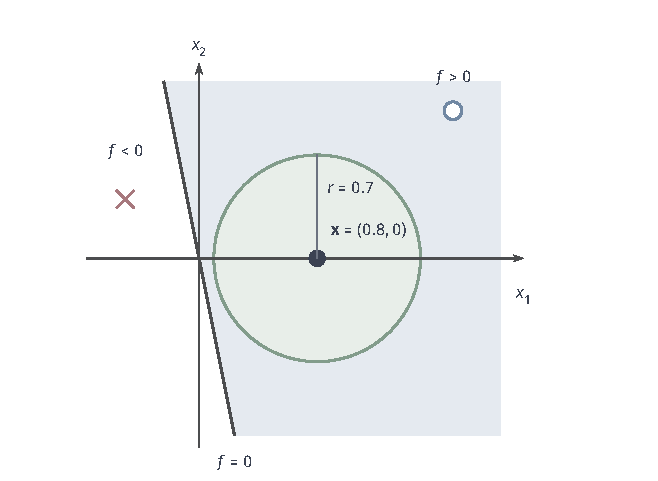
\includegraphics[width=\linewidth]{figures/03-foundations/03-trustworthiness/tikz/trust-certified-region/figure.pdf}
  \caption{教学分数$f(\bm x)=x_1+0.2x_2$在$(0.8,0)$取0.8，$L=\sqrt{1.04}$，$r=0.7$满足$0.8>Lr$，故闭球内符号正。深线为零边界，球外空心点正、叉点负；球外不受这份证书判定。证书保证符号保持，未判原标签正确。}
  \label{fig:trust-certified-region}
\end{figure}

直接对复杂模型给出有用的变化上界往往太宽松，于是出现了一条“先构造一个便于认证的新分类器，再给新分类器发证”的思路。\term{随机平滑}（randomized smoothing）就是代表：不给原分类器$h$直接发证，而是先在它的输入上注入高斯噪声、对噪声下的预测进行投票，以得票最高的类别作为新分类器$g$的输出，平局按预先固定的规则裁决：
\begin{equation}
 g(\bm{x})=\arg\max_k
   \mathbb P_{\bm{\varepsilon}\sim
   \mathcal N(\bm{0},\sigma^2\bm I)}
   \{h(\bm{x}+\bm{\varepsilon})=k\}.
 \label{eq:robustness-smoothing}
\end{equation}
其中$\bm{x}\in\mathbb R^d$，$\bm I$是$d$阶单位阵，$\sigma>0$是注入噪声的标准差。这样构造的直觉是：投票把许多带噪预测聚合起来，输入发生小变化时，噪声云团只是轻微平移，各类的得票概率变化平缓、可以用高斯分布精确刻画，于是可认证性来自这种平滑性而非原模型。Cohen 等利用高斯分布平移时分类区域概率的变化关系，为平滑后的分类器$g$建立了$\ell_2$扰动下的证书\scite{cohen2019smoothing}。注意认证对象始终是新规则$g$，不是原模型$h$。

记$\underline p_a\in[0,1]$为胜出类别$a$的投票概率下界，$\overline p_b\in[0,1]$为其他每个类别投票概率的共同上界。当$\underline p_a>\overline p_b$（$a$的得票严格且有间隔地领先）时，利用两个高斯分布平移后概率质量的关系，可以推出一个扰动半径，半径内$a$必然保持胜出：
\begin{equation}
 \lVert\bm{\delta}\rVert_2<r_{\mathrm{cert}},
 \qquad
 r_{\mathrm{cert}}
 =\frac{\sigma}{2}
 \left[\Phi^{-1}(\underline p_a)
       -\Phi^{-1}(\overline p_b)\right]
 \label{eq:robustness-smoothing-radius}
\end{equation}
其中$\Phi$是标准正态分布函数，$\Phi^{-1}$是其分位函数，端点0和1按极限理解。这个半径保证的是投票规则：对半径内的任意扰动，平滑分类器的输出类别都是$a$。它既不保证某一次带噪声的$h$预测正确，也没有给原模型直接发证。

实际中各类的投票概率未知，只能用蒙特卡洛抽样估计，并且必须使用有效的置信界把抽样误差计入证书。举例说明量级：二分类若已知$\underline p_a=0.9$，则可令$\overline p_b=0.1$，取$\sigma=0.25$时认证半径约为$\frac{0.25}{2}[\Phi^{-1}(0.9)-\Phi^{-1}(0.1)]=0.25\,\Phi^{-1}(0.9)\approx0.25\times1.282\approx0.32$。这里的0.9必须是有置信保证的下界，90\%的经验票数不能直接当作0.9。还有一个选择偏差要处理：用同一批样本既选出胜出类别、又估计该类概率会导致界失效，必须为选类和估概率分别独立采样，或采用对选择同时有效的程序；当抽样不足以把胜出类与其他类分开时，正确做法是拒绝认证，而不是硬给一个半径。

增大噪声强度$\sigma$并不一定让证书更实用。$\sigma$在公式里是乘性因子，但改变噪声也会改变各类投票概率。更强噪声可能缩小胜出类与其他类的概率间隔，也可能损害分类正确率，却没有一般的单调规律。因此不能固定住概率界，只看式中的$\sigma$就断言半径变大，而须重新估票、认证并评价准确率。此外平滑要为每个输入做多次前向计算，成本显著增加。因此报告时至少要同时给出认证准确率随半径变化的曲线、计算成本和认证失败的比例；其中认证准确率计数的是“预测正确且证书覆盖指定半径”的样本比例。还要注意，单样本证书上的置信界并不自动保护一整批样本或整条曲线上的所有点，若要对整批或整曲线下联合结论，必须为每个点分配失败概率或做联合控制。这种随机性来自估票抽样，与上一章校准检验、共形覆盖所依赖的“校准样本加新样本”随机性是不同对象。

有了逐样本证书后，如何汇总成一个总体指标？给定目标开球半径$r$，对每个样本检查两件事是否同时成立：预测正确、且认证半径不小于$r$；满足的样本占比就是该半径下的认证准确率。也可以把搜索与认证并列报告搜索鲁棒准确率：搜索若找到反例则判该样本失败，证书若成功覆盖则判稳定，两者都没有结论时保留“未判定”而不是强行归类。无论哪种汇总，逐点证书本身都不保证测试样本能代表未来总体，要把它升级为总体风险结论，仍需回到抽样条件。

\subsection{变化识别与拒绝效果的检验}
\label{sec:robustness-monitor-test}

无论风险测试还是邻域认证，都只覆盖事先声明的范围。当输入落到范围之外，另一条防线是让系统识别出来并报警、转交人工，从而限制模型的使用。这里要分开检验两件事：一是识别“输入已离开熟悉范围”的能力，二是识别之后实际损失降低了多少。这两项证据支持的是系统层面的止损，并不证明分类器在这些输入上仍然正确——恰恰相反，拒绝往往意味着承认模型在这里不可靠。

\term{分布外检测}（out-of-distribution detection，简称 OOD 检测）要判断一个输入是否来自训练分布之外。做这件事必须先有三个参照物：预设的域内分布是什么、检测的输入单位是什么（一封邮件、一张图还是一个会话）、以及“域外”由哪些备择来源代表。这几个对象容易混淆：训练时没见过的语义新类别、输入边缘分布改变的协变量变化、以及域内本身就罕见的低密度困难样本，是三种不同情况，用实验中某个域外数据集的标签，只代表那一个选定来源，不代表一切未知。检测可用输入到训练集的距离、密度估计，或模型输出的各种分数做异常程度度量并选择阈值，但要警惕两个直觉错误：低密度不等于难预测（罕见但规则明确的输入可能很好分），高置信也不等于熟悉（模型可以对陌生输入自信地错）。因此检测必须按漏检（放进来域外输入）和误报（拒绝正常输入）的成本来评价；仅凭有限的参考数据，也不可能识别任意形式的未知分布。

检验流程上，先固定异常分数的定义，再分别保留三份数据：正常的域内资料、预先指定的未知类别或来源，以及一份完全独立的验证集用来选阈值；最后在测试集上报告两类错误——误拒正常输入的比例和误接纳未知输入的比例。排序类曲线（如 ROC）适合比较不同分数的整体区分力，但选定实际工作点时必须结合两种错误的具体成本。曲线下面积本身没有直接计入成本；像 FPR95 这类指标还要核对方向和分母：若把域内定义为正类，FPR95 表示保留 95\% 域内输入（只拒绝 5\%）时，域外输入被错误接纳的比例，引用前必须确认它说的到底是哪一侧。

识别准确不等于止损有效：熟悉的输入也可能分错，陌生的输入也可能恰好分对。要评价拒绝是否真的减少了损失，必须另取任务标签，计算上一章定义的接受风险、总体处理比例和转交成本，并在相同处理量或相同成本下比较不同规则。这样，第~\ref{chap:trust-reliability}章的选择性预测检验就与检测接了起来：用域外标签检验“陌生的能否被识别”，用任务标签检验“拒绝之后错误是否真的下降”。第~\ref{sec:robustness-rejection}节还会具体构造检测分数。

分布外检测针对单个输入是否陌生，\term{漂移检测}（drift detection）则针对一段数据流：观察数据的统计关系是否随时间发生了改变。要特别注意输入分布改变与风险改变之间没有必然联系：输入边缘分布变了，模型若不依赖变化的部分，风险可能毫不动；反过来，输入边缘分布看起来稳定，也可能掩盖了标签条件关系的改变。因此在缺少标签时，漂移信号只能作为“启动调查或暂时收窄使用”的触发器，它本身不能决定新模型该往哪个方向更新。

用两个对比例子说明这种分离。模板占比的改变很容易被输入特征的统计检验发现，但如果模型本来就不靠模板分类，风险未必增加；而发件主体被接管时，输入的边缘分布几乎不变（还是那些地址、那些措辞），标签关系却已经改变，纯输入漂移检测可能完全无动于衷。要把输入信号与真实错误、行动损失对应起来，最终仍需要持续获得少量真实标签。上一章的统计区间在这里照样要匹配真实抽样结构；任意反复查看、靠同一批监测数据挑出来的“漂移点”，不能直接套用为固定一次检验设计的区间。

评价报警机制时应保留时间顺序，把已知无变化的时间段和有变化的时间段分开，分别测量误报率、漏报率和发现延迟，并完整保存窗口长度、阈值和重置规则，结果才可复现。真实部署中变化起点通常未知，此时只能报告“已核实的统计差异”及差异出现后的风险，不能把所有报警都算作真阳性——有些报警只是噪声。等延迟返回的标签把真实风险补齐后，再另行核算“因为报警而拒绝或更新”到底带来了多少收益和代价。

\section{鲁棒性的增强}
\label{sec:robustness-enhancement}

增强方法的选择应由诊断决定，而不是把所有手段堆在一起。对应前面的失效机制：标签保持的局部错误，需要约束模型对输入变化的行为；困难群体被平均忽略或环境中存在捷径，需要调整训练风险和所依赖的依据；范围外输入信息不足，需要拒绝；而新环境确实带来了可用信息时，才考虑让模型适应。前三类措施不要求在部署中持续改变模型参数，适应则要额外处理状态更新、错误累积和旧能力遗忘，因此风险也不同。这些措施可以组合，但评价时要分清各自改变了什么。

在着手增强鲁棒性之前，先排除一个平行问题：数据污染。个别标注错误或测量异常会产生极大的残差，把模型往错误方向拉。Huber 损失在残差较小时使用平方项、残差较大时改为线性项，从而限制单个异常点的影响；其他稳健损失或迭代降权也有类似作用。但机械降权有一个伦理与正确性上的风险：合法的少数群体也可能天然残差较大（因为它们在训练数据中本就代表不足），把它们当噪声压下去，会进一步牺牲这些群体。因此异常标签、测量噪声与“模型还没学会的合法样本”必须靠数据诊断区分，不能只凭残差大小处理。

\subsection{输入变化下的行为约束}
\label{sec:robustness-local-enhancement}

最直接的增强思路，是把任务预期的标签保持变换$T$直接放进训练，用$\ell(f(T(\bm{x})),y)$要求模型对变换后的输入仍预测原标签。在没有标签的场景（如无监督一致性训练），可以改为约束变换前后的概率、分数或中间表示彼此接近，但必须明确用什么量衡量差异、权重多大。这里的前提是变换真的保留任务含义：若把一致性约束加得过强，会把本来有意义的差异也强行抹掉（例如把“否定词被删”这类改变语义的变化也当成应保持）。

除了约束“同一样本的变换前后”，还可以约束“不同样本之间”的函数变化。\term{混合增强}（mixup）用同一个权重对两个输入和它们的标签分别做线性插值。设$\bm{e}_y$为类别$y$的独热标签，则混合样本和混合标签为
\begin{equation}
 \begin{aligned}
  \widetilde{\bm{x}}&=\lambda\bm{x}_i+(1-\lambda)\bm{x}_j,\\
  \widetilde{\bm{y}}&=\lambda\bm{e}_{y_i}
                         +(1-\lambda)\bm{e}_{y_j},
 \end{aligned}
 \label{eq:robustness-mixup}
\end{equation}
其中$\lambda\in[0,1]$是输入和标签共用的插值权重，通常从对称的 Beta 分布中随机抽取。用软标签交叉熵训练时，两类的损失按$\lambda$和$1-\lambda$的比例分担，并不强迫这个“介于两者之间”的样本一定属于某个端点类别\scite{zhang2018mixup}。

当两个端点类别不同时，例如$\lambda=0.7$，混合标签就是在两类上的概率向量$(0.7,0.3)$；训练要求模型在看到 70\% 的甲样本与 30\% 的乙样本混合而成的输入时，输出也接近这个概率向量。这种做法在样本之间增加了一条平滑的形状约束，但它依赖一个语义假设：插值出来的点应当是“有意义”的。对图像，两张图按像素线性混合通常还能看出内容；对邮件这类离散文本，按字节混合两封信往往产生毫无意义的乱码，在表示空间插值是否合理也需要单独核验。更重要的是，端点标签正确并不自动证明中间的软标签就是真实标签分布，因此它与式~\eqref{eq:robustness-perturbation-risk}那种“标签保持的邻域”是两种不同对象，不能混为一谈。

AugMix 走的是另一条路：从同一张图像出发生成多条随机增强链，把这些视图混合起来并保留原图通路，还可以训练模型对各视图给出一致预测\scite{hendrycks2020augmix}。它约束的是“同一对象在合理变化下的表现应当一致”，并不规定不同类别之间存在线性过渡。

由此可以看清两种方法的假设差别：mixup 比较的是不同样本之间的过渡，AugMix 比较的是同一样本的多个合理视图。检验时必须保留各自的假设，不能笼统地说“增强数据就更鲁棒”。增强前要检查小目标、关键颜色或文字方向有没有被增强破坏；增强后要用训练时没有用过的损坏类型及其组合复查迁移效果，否则测到的只是对所选增强的拟合。

随机增强还有一个覆盖问题：随机抽到的大多是“容易”的变化，可能恰好漏掉允许邻域中少数让模型严重出错的位置，而那些位置才是式~\eqref{eq:robustness-perturbation-risk}中上确界关心的。最不利训练主动去寻找这些高损失位置并在那里施加压力，但过分追逐最坏点也可能扭曲原本正常的数据边界。鲁棒零一错误可以分成两种互斥情形：原输入已经分错；原输入分对，但允许邻域内存在分错的变体。前者需要改善干净分类，后者需要减少邻域内可触发的错误。TRADES的理论分析通过分类校准损失及相应转换，把这两部分与可优化的代理量联系起来，为同时兼顾分类拟合与局部稳定的目标提供依据\scite{zhang2019trades}。

令$\bm{p}_{\bm{\theta}}(\bm{x})$表示模型输出的多类别概率分布，$\bm{\theta}$为参数向量、$\Theta$为候选参数集，$\mathcal P_{\mathrm{train}}$为训练数据的联合分布。TRADES 在原输入上使用负对数似然损失，在邻域上使用预测分布之间偏离程度的上确界，目标写为
\begin{equation}
 \begin{aligned}
 \min_{\bm{\theta}\in\Theta}\
 \mathbb E_{(\bm{x},y)\sim\mathcal P_{\mathrm{train}}}
 \bigg[&-\log p_{\bm{\theta},y}(\bm{x})\\
 &+\beta\sup_{\bm{x}'\in U(\bm{x})}
 D_{\mathrm{KL}}\!\left(
 \bm{p}_{\bm{\theta}}(\bm{x})
 \,\middle\|\,
 \bm{p}_{\bm{\theta}}(\bm{x}')\right)\bigg],
 \end{aligned}
 \label{eq:robustness-trades}
\end{equation}
实现时外层期望用样本平均近似，$\beta>0$控制稳定性项相对于分类项的权重，$D_{\mathrm{KL}}$是 KL 散度，衡量两个类别分布的差异。两项各管一件事：第一项要求模型在干净输入上把真实类别的概率抬高；第二项惩罚模型在允许邻域内出现的最大预测变化，即专门盯住最容易被扰动改变预测的位置。内层上确界通常只能用有限步搜索近似，因而拿到的是偏离的一个下界近似。还要注意它与鲁棒零一风险之间的距离：这里的交叉熵加KL是沿理论动机构造的训练代理，其原始数值不能直接解释为鲁棒零一风险上界。原论文的风险界还包含校准转换、最优自然风险与最优代理风险等量，实现使用了便于优化的替代形式；从代理下降到风险受控，仍须核对损失条件、推广误差和内层求解误差。如果去掉分类项、只保留稳定项，对所有输入输出同一分布就能让KL为零，却不能据此保证模型正确区分任务类别。

训练前还要核验邻域定义本身是否自洽。如果两个不同类别的样本在规定邻域内互相重叠，那么“各自的标签保持邻域”这两个要求就直接冲突——同一个点会被要求同时属于两类，这种矛盾不能靠调大$\beta$解决。先确认范围相容，再选择$\beta$；即便如此，内层搜索仍增加训练计算，而且训练目标数值下降并不等于获得了形式化证书。对抗扰动的搜索与梯度遮蔽等更细致的检验留到第~\ref{chap:trust-security}章。

图~\ref{fig:trust-adversarial-training-loops}把式~\eqref{eq:robustness-trades}的内外两层拆开：内层固定参数，在邻域$U(\bm x)$中寻找使原预测与扰动预测 KL 散度最大的扰动；外层再用干净输入的分类损失加加权的 KL 项更新参数，随后重新搜索。内外交替进行。需要强调，内层搜索产生的只是“当前找到的最坏候选”，并没有证明它是全局最坏点。

\begin{figure*}[htbp]
  \centering
  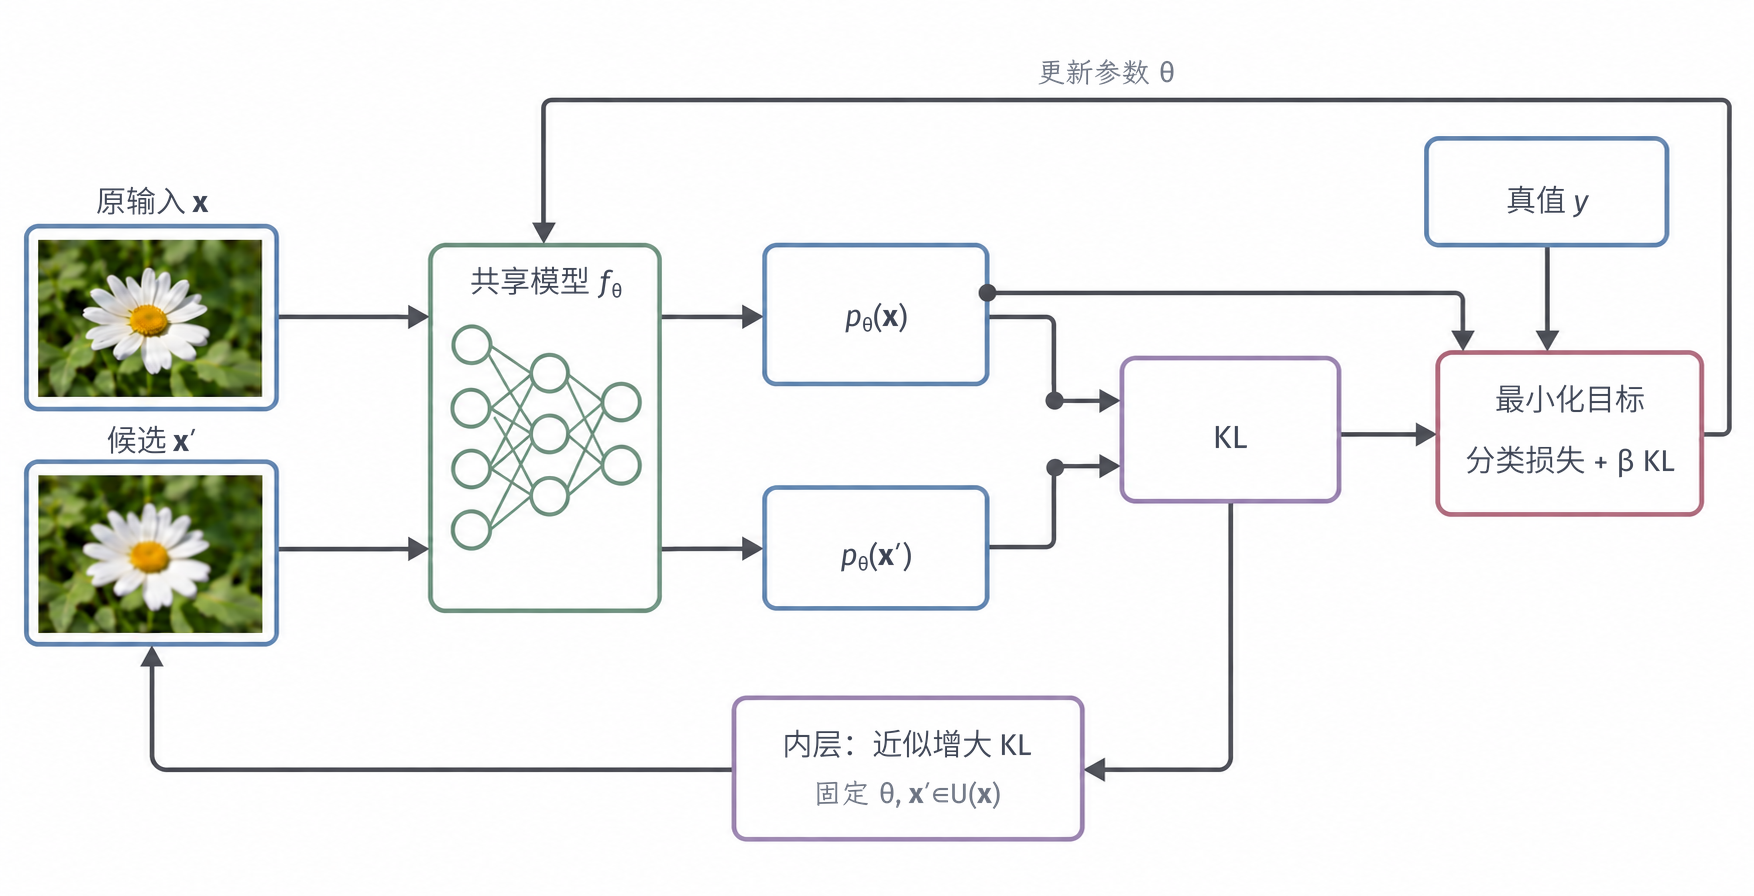
\includegraphics[width=164.600mm]{figures/03-foundations/03-trustworthiness/generated/adversarial-training/figure.png}
  \caption{TRADES内层固定参数，在$U(\bm x)$近似增大原、扰动预测之间的KL；外层最小化原输入的分类损失与加权KL，再重新搜索。共享模型分别处理两输入，原预测还独立进入分类损失。数字样本和箭头均为示意，未提供实际扰动大小或全邻域形式证书。}
  \label{fig:trust-adversarial-training-loops}
\end{figure*}

鲁棒性常被说成“免费”或必然牺牲准确率，图~\ref{fig:trust-robust-accuracy-tradeoff}用一个固定样本和扰动的教学比较澄清这种取舍。四个候选模型中，A、B、C 的干净准确率依次升高（80、88、94），鲁棒正确数却依次下降（70、60、45），确实呈现取舍；但 D 干净90、鲁棒74，两项都优于 B。因此图中虚线只连接 A、B、C 以展示一种可能的取舍，它不是所有任务上都成立的最优边界：改进训练完全可能同时改善两者，是否存在真实取舍必须在固定样本、固定邻域和搜索条件下比较。

\begin{figure*}[htbp]
  \centering
  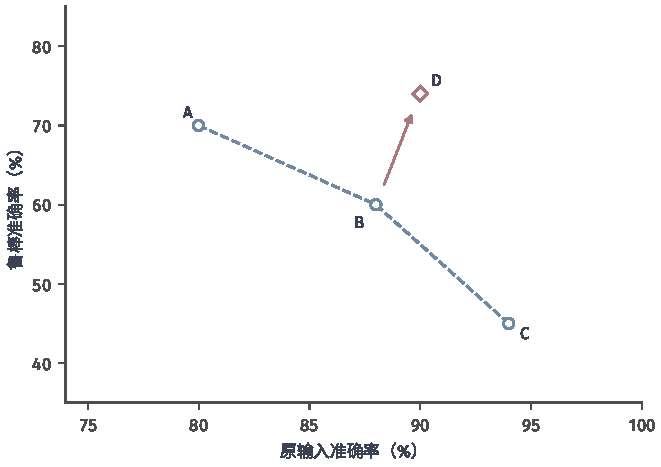
\includegraphics[width=112.000mm]{figures/03-foundations/03-trustworthiness/matplotlib/trust-robust-accuracy-tradeoff/figure.pdf}
  \caption{固定100个教学样本和标签保持邻域，原输入、鲁棒正确数依次为A 80/70、B 88/60、C 94/45、D 90/74。鲁棒正确是原正确子集，D两项优于B。虚线仅连A、B、C，不是实验或普遍最优边界；比较还需共同扰动及搜索条件。}
  \label{fig:trust-robust-accuracy-tradeoff}
\end{figure*}

最后回到证据纪律：改变训练约束后，仍要按第~\ref{sec:robustness-risk-test}节在独立数据上测试；若声称严格邻域稳定，则要另用第~\ref{sec:robustness-certification}节的认证。训练目标的数值降得再低，也不能直接推出证书半径变大——前者是经验优化量，后者是形式化保证。

\subsection{跨环境风险与稳定依据的约束}
\label{sec:robustness-environment-enhancement}

局部邻域约束既没有改变不同环境在训练中的权重，也没有判断模型依赖的依据能否跨环境成立。当问题出在困难群体被平均目标忽略、或预测关系本身随环境变化时，需要换一个层次的做法：保持损失定义不变，但扩大训练目标所覆盖的环境，并明确希望模型依赖的、跨环境保持的预测关系到底是什么。

先按任务规定一个允许分布族$\mathfrak Q$：例如允许已声明的各环境以任意比例混合，或允许真实分布在参考分布周围某个预设距离内变化。\term{分布鲁棒优化}（distributionally robust optimization, DRO）不再最小化平均风险，而是比较每个候选模型在族内最坏环境下的风险，从模型族$\mathcal F$中选出把这个最坏风险压得最低的模型。监督学习下的目标为
\begin{equation}
 \min_{f\in\mathcal F}\ \sup_{\mathcal Q\in\mathfrak Q}
   \mathbb E_{\mathcal Q}\ell(f(\bm{x}),y).
 \label{eq:robustness-dro}
\end{equation}
式~\eqref{eq:robustness-dro}把每个候选模型在允许分布族内的最高期望损失作为比较依据，即“先对环境取最坏，再在模型中选最优”（这种极小极大结构可参考\BookChapterRef{chap:decision-theory-and-dynamic-risk}{卷2《数学准备：概率、因果与决策》第6章“策略的价值与优化”}）。要强调的是，DRO 首先是一个训练或压力测试目标：用它训出的模型仍须独立测试，目标值本身并不给部署程序提供任何证书。若想进一步得到高概率的风险上界，需要额外的统计构造：从抽样来源明确的训练集$S=\{(\bm{x}_i,y_i)\}_{i=1}^n$出发构造一个数据驱动的不确定集合$\widehat{\mathfrak Q}(S)$，用独立资料或预先固定的统计规则选择距离、矩约束、半径或分组，并证明对随机样本$S$，真实分布以至少$1-\delta$的概率落在$\widehat{\mathfrak Q}(S)$内；再把这层“包含关系”与经验推广误差、内层上确界的近似误差合在一起，才能转成最终风险界。集合设得太小会漏掉真实变化，设得太大又会包含毫无意义的压力情形，使优化过于保守；分布的可积性、上确界能否取到、以及如何近似，都会影响保证是否成立。

在一种重要的特殊情形下，DRO 会简化成很直观的形式。如果只允许若干个组分布以任意比例混合，那么最不利分布会把全部权重放在风险最高的那个组上，式~\eqref{eq:robustness-dro}就退化为“最大组风险最小化”。它能防止大组的低风险在平均中压过小组的高风险，但并不消除组内自身的泛化误差。Sagawa 等指出，过参数模型甚至可以同时把所有训练组的误差都拟合到零，但最坏组在新数据上的泛化仍需配合正则和专门的验证\scite{sagawa2020groupdro}。

具体推导如下。设共有$G$个组，组$g$的分布为$\mathcal P_g$，组内风险为$R_g(f)=\mathbb E_{\mathcal P_g}\ell(f(\bm{x}),y)$。给定混合比例$q_g\geq0$、$\sum_gq_g=1$时，混合风险是各组风险的加权和$\sum_gq_gR_g(f)$。若允许任意比例（$\bm q$取遍单纯形），把全部权重放到风险最高的组即取得上确界：
\begin{equation}
 \sup_{\bm{q}\in\Delta_G}\sum_{g=1}^{G}q_gR_g(f)
       =\max_{1\leq g\leq G}R_g(f),
 \label{eq:robustness-group-dro}
\end{equation}
其中$\Delta_G=\{\bm q\in\mathbb R^G:q_g\geq0,\ \sum_gq_g=1\}$是$G$个非负分量之和为1的概率单纯形，仿射维数为$G-1$。这个等式解释了组 DRO 的取向：示例~\ref{ex:robustness-mixture}中，普通平均目标主要由占 99\% 的常见模板决定，少见模板几乎没有话语权；而最大组目标会首先盯住少见模板那 50\% 的错误率，强迫模型先解决最差的组。

计算上可以交替进行：增大当前高损失组的权重，再更新模型，如此往复。如果担心“任意比例”过于保守，也可以只允许混合比例在当前比例附近，以减轻极端加权。使用中有三个实际问题：分组太粗会漏掉组内的捷径，分组太细又使每组样本太少、估计剧烈波动，而组标签本身未必总能拿到；若按“哪些样本损失高”自动分组，还容易把标注错误样本混进“困难组”，需要额外的数据诊断，优化目标本身分不清一个高损失样本是合法的困难群体还是脏数据。

还要划清一条边界：把各组风险都压低，并不自动等于机会或成本的分配是公平的；即使各组错误率相等，也可能只是“一样地差”，或者这些错误对不同组的后果完全不同。第~\ref{chap:trust-fairness}章会先确定分配原则，再判断哪些差异真正有意义。本节的组 DRO 只在既定损失和既定分组上做优化，不能据此声称模型已经公平。

多个环境提供的另一种价值，是帮助识别跨环境稳定的依据：如果某条关系在所有环境中都成立，它更可能是可迁移的。但这有前提——环境集合必须足够多样，足以打破那些不稳定的关系；仅凭多个环境上的训练表现一致，并不能保证在任意新环境成立。第~\ref{sec:domain-generalization}节讨论从不变性到目标域保证所需的条件。

这里区分两种常见目标。不变风险最小化（IRM）寻找一种表示，使同一个预测规则在所有训练环境上都同时最优；组 DRO 则只约束最坏组的损失，并不要求各组的最优规则彼此一致。两者都可能被“同向捷径”骗过：如果所有训练环境中模板与标签都同向相关，IRM 也可能把模板当成不变量。反过来，若各环境的真实最优规则本来就不同，强迫共用一条规则还会丢失合理的环境特异信息。

评价这些复杂目标时，基准必须公平。DomainBed 在七个多域数据集上用统一实现比较了九种方法和三类模型选择准则，结果报告普通经验风险最小化（ERM）在这些设置下取得了当时领先的目标域准确率\scite{gulrajani2021}。这说明方法名字带来的直觉不能替代在相同条件下认真训练、调优和验证的比较——一个调参充分的简单基线往往很强。

当然，DomainBed 的结论只限于它比较过的数据集和设置，不能反过来说 ERM 在一切变化下都最优。正确的评价方式是固定架构、训练预算、增强方式和可见的验证环境，只改变训练目标，才能把收益归因到目标本身。第~\ref{chap:transfer-learning-theory}章回答“信息何时足以识别可迁移规律”，受控实验则进一步检查具体算法有没有效利用这些信息，两者缺一不可。

\subsection{超出适用范围时的拒绝策略}
\label{sec:robustness-rejection}

当数据中的信息根本不足以覆盖所有可能输入时，再怎么训练也无法对域外输入作出可靠承诺。此时现实的做法是提高“接纳条件”：只在模型足够有把握时才自动给出预测，否则交给人工。要清楚拒绝增强的是系统的变化应对能力，而不是被拒输入上原模型的准确性——拒绝并未证明原模型在被拒输入上更准确，只是不再自动执行这部分决定。被拒输入也可能恰好能被分对，拒绝理由应是证据、风险容限或适用范围，而不是未经检验就断言模型一定不会处理。因此报告时要把处理量的减少和人工负担的增加，与模型质量的收益分开记录。

最简单的熟悉程度分数是\term{最大类别概率}（maximum softmax probability, MSP）：直接取 softmax 输出向量中的最大概率，低于阈值就拒绝。Hendrycks 与 Gimpel 把它作为错误样本和分布外样本检测的基线，好处是无需重新训练模型\scite{hendrycks2017msp}。

MSP 的弱点在于它只看各类别之间的相对差异，丢弃了归一化之前的幅度信息。看一个具体构造：两个输入的未归一化分数（logits）分别为$(10,9)$和$(1,0)$，两组数的差都是1，softmax 之后最大概率同为$e/(e+1)\approx0.731$，MSP 给它们相同的熟悉分数；两组logit只相差一个加到所有类别上的公共常数，类别间差值相同，所以softmax和MSP完全相同。仅靠分类概率或交叉熵目标，不能把这项公共幅度解释为判断更强或更弱。能量分数可以保留幅度差，但它是否对应所选域外来源仍须另验。此外，“域外”的语义和测试分布需要另行定义，模型在原类别上是否校准，也没有验证过它能否代表陌生程度。

若想保留归一化之前的幅度信息，可以从$K$个类别的实值分数$z_k(\bm{x})$和温度$T>0$构造\term{能量分数}（energy score）：
\begin{equation}
 E_T(\bm{x})=-T\log\sum_{k=1}^{K}
       \exp\!\left(\frac{z_k(\bm{x})}{T}\right).
 \label{eq:robustness-energy}
\end{equation}
在固定模型与预设备择来源的检测中，常把较大的能量作为域外信号。能量的符号和范围受logit公共偏移影响，并不总是负数，“更大”也不等于“更接近0”；阈值与方向仍应由独立验证记录确定。Liu 等比较了直接用能量检测，以及在训练中显式拉开域内与域外输入能量的方案\scite{liu2020energy}。

在$T=1$时，前面两个向量的能量分别约为$-10.313$和$-1.313$，差异被保留下来，MSP 无法区分的两点现在可以区分。但要立刻补上边界：能区分这两个点，不等于能量高低就对应“未知的程度”。给所有类别的分数加上同一个与输入有关的常数，会改变能量却完全不改变 softmax 概率——这说明仅凭分类训练目标，输入空间上的密度并不能被唯一确定，能量不是真正的输入对数密度（除非额外做生成式拟合）。因此能量阈值仍须在实际模型和实际备择数据上验证，不能直接当作密度使用。

如果能获得一批辅助的异常数据，还可以用\term{异常暴露}（outlier exposure, OE）让模型在训练时就“见过异常”：在正常任务损失之外，增加一项对任务外输入的约束。一种分类实现是让模型对异常输入输出接近均匀的分布，避免它对陌生样本也给出尖锐的类别判断\scite{hendrycks2019oe}。

异常暴露的关键限制是：辅助异常不可能代表全部未知来源，而且如果同一批异常数据既用于训练又用于测试，模型可能只学会识别这批数据的来源线索，而非真正的陌生性。应当留出训练时没见过的异常类别和来源，在测试前固定好各组。对邮件任务可以预先指定两类不同的备择：把从未见过的诈骗模板来源作为“与域内较相似”的备择，把非邮件文档（如纯文本表格）作为“差异明显”的备择；但这两组都只是预先选定的检验来源，不构成对未知的完备覆盖。按第~\ref{sec:robustness-monitor-test}节的要求冻结阈值、独立检验后，应分别报告各组输入被误接纳的比例。

\subsection{利用新环境信息时的风险与验收}
\label{sec:robustness-adaptation}

前三类增强都不要求模型在部署中改变自己；最后一类不同：新环境不断产生数据，模型可以利用这些数据在线改变运行状态，例如重估某些统计量、做部分参数更新，或把当前模型的高置信预测当作伪标签（pseudo-label）反过来参与训练。\term{测试时适应}（test-time adaptation）就是这类方法的统称；具体算法与训练过程可参考\BookChapterRef{chap:ket-transfer-adaptation}{卷8《学习范式：知识的获取、演进与迁移》第12章“知识的迁移与适应”}，本节只检查它怎样改变可靠性主张、以及验收需要什么条件。

无标签适应最大的风险是：没有真实标签，更新方向只能依赖一些代理信号，如预测置信度、增强前后预测的一致性。但代理改善不等于任务风险下降——模型可能把自己的错误预测通过高置信伪标签不断强化（自证循环），也可能因为对所有输入都输出常数而显得“一致性很好”。限制可更新的参数范围、步长和每批样本数量，可以缩小出错时的影响范围，但并不能证明更新方向正确。只要能拿到少量真实标签，就应优先用它核验真实任务表现，而不是只盯着代理指标是否改善。

适应模型还有一个离线评估容易忽略的特点：它的输出依赖自身状态，而状态受处理历史影响。批次如何划分、样本以什么顺序到达、对一个输入是先预测还是先更新、何时把状态重置，都会使完全相同的输入在不同时刻面对不同的模型状态，这些都属于必须明确的程序定义。把数据顺序打乱后做离线适应，不能代表时间相关的真实服务；只评价发生了高置信更新的那部分样本，也会系统性遗漏其余输入和困难群体。

因此评价适应程序时，应让冻结的对照模型与适应模型在同一条时间流、同样的计算预算下并行运行，报告两者在新环境和旧环境上的风险、风险随时间的变化轨迹、关键组表现、回退是否有效，以及更新计算和状态保存的成本。部署前还要事先写死一组规则：新环境的风险容限是多少；相对于冻结参照，旧环境和关键组的风险最多允许增加多少；连续几个时间窗越界就触发动作；回退到哪个版本；用什么资料复验。总体平均收益不能抵消某个短时间窗的严重退化，新环境的收益也不能掩盖旧能力的遗忘，这两条都要用预设规则约束，不能事后解释。

当标签不足以判断更新方向是否正确时，稳妥的处置是保留冻结参照、收窄自动处理范围或直接回退，以避免模型沿着错误的代理信号继续优化。这些处置本身并不证明适应成功，它们只是止损。只有把模型版本、更新规则、运行状态和验收条件全部固定下来，观察到的结果才能归因于完整的适应程序，而不是某个偶然的状态轨迹。

\section{本章小结}
\label{sec:robustness-summary}

本章把两类问题严格分开：一是变化之后模型本身的表现如何，二是证据不足时系统怎样止损。变化条件来自三个层次——输入测量扰动、群体比例改变、特征与标签规律改变；需要诊断的典型机制包括决策边界过近、困难组占比上升与捷径依据失效。这不是一一对应的分类，同一种变化可能同时暴露多种机制，明确实际路径后才能选择补救。检验上，受控损坏基准、跨来源测试回答的是平均风险，局部证书回答的是指定邻域内不翻转，分布外检测、漂移监测、拒绝和回退回答的是范围外能否止损；它们的证据对象不同，任何一种都不能替代其余判断。

增强方法按改变的对象分类：数据增强与局部稳定训练约束模型对输入变化的行为，分布鲁棒优化（包括最大组风险）改变训练风险对环境和群体的加权，范围外拒绝不改变模型而只收窄它的自动决定权，测试时适应则用新环境信息更新运行状态，同时承担错误自我强化和旧能力遗忘的风险。与调优充分的基线比较之后，任何方法都仍需同时检查原环境、新环境、关键组与资源代价；当更新的证据不足时，应收窄使用而不是强行部署。

回到开篇的误拦事故，排查路径现在很清楚：先判断变化发生在测量、群体比例还是标签关系，再对应检查决策边界、原本就存在的高错误组和模型对模板的依赖，据此取得补救所需的信息。如果排查发现损失集中在某个人群，还要进一步追问这种负担分配是否合理——这正是下一章公平性要处理的问题；而“模型究竟用了哪些因素作判断”，则由第~\ref{chap:trust-interpretability}章的解释方法进一步回答。

\paragraph{扩展阅读}

常见损坏基准与WILDS分别提供受控扰动和真实来源差异的证据。对照阅读时保留类型、划分及模型选择条件，就能确定基准平均结果适用到哪里\scite{hendrycks2019corruptions,koh2021wilds}。

TRADES与组DRO分别针对局部稳定和最大组风险；测试时适应的状态、算法与实践仍需结合适应条件核查\scite{zhang2019trades,sagawa2020groupdro}。
